\documentclass[UTF8,a4paper,12pt]{ctexart}

\usepackage{amsmath,amssymb}
\usepackage{booktabs}
\usepackage{caption}
\usepackage{float}
\usepackage{geometry}
\usepackage{graphicx}
\usepackage{hyperref}
\usepackage{longtable}
\usepackage{xcolor}
\usepackage{enumitem}
\usepackage{fvextra}

\geometry{left=2.6cm,right=2.6cm,top=2.6cm,bottom=2.6cm}
\hypersetup{colorlinks=true,linkcolor=black,urlcolor=blue}
\setlength{\parindent}{2em}
\setlength{\parskip}{0.25em}
\setlength{\emergencystretch}{3em}
\linespread{1.25}
\setlist[itemize]{leftmargin=2.5em,itemsep=0.15em}
\DefineVerbatimEnvironment{CodeBlock}{Verbatim}{breaklines,breakanywhere,fontsize=\small,frame=single,rulecolor=\color{gray!45}}

\title{\heiti 机器学习与Python实践\\[0.8em]\Large 第2次作业\\[1.6em]\Huge 共享单车小时租借数量预测}
\author{}
\date{}

\begin{document}

\begin{titlepage}
    \centering
    \vspace*{1.2cm}
    
\includegraphics[width=0.78\linewidth]{figures/cover_logo.png}\par
    \vspace{1.0cm}
    {\zihao{2}\heiti 机器学习与Python实践\par}
    \vspace{0.8cm}
    {\zihao{3}\heiti 第2次作业\par}
    \vspace{1.2cm}
    {\zihao{1}\heiti 共享单车小时租借数量预测\par}
    \vfill
    \begin{tabular}{rl}
        姓名： & 匿名\\[0.45em]
        专业： & 强基班\\[0.45em]
        学号： & \\[0.45em]
        教师： & 匿名\\[0.45em]
        学院： & 信息科学与工程学院\\[0.45em]
    \end{tabular}
    \vfill
    {\zihao{4}2026年05月22日\par}
\end{titlepage}

\tableofcontents
\newpage

\section{前言及问题概述}

共享单车系统是城市短距离出行中的重要组成部分。用户可以在不同地点租借和归还自行车，系统会记录每一次租借发生的日期、小时、天气、温度、湿度、风速和用户类型等信息。由于骑行需求受到时间规律、工作日与节假日、天气条件以及季节变化等多种因素影响，若能够根据这些环境和时间特征预测每小时租借数量，就可以为车辆调度、站点补车和运营维护提供参考。

本次实验围绕华盛顿 2011--2012 年每小时共享单车租赁数据展开。预测目标为 \texttt{cnt}，即每小时租借自行车总数。实验流程与题目要求保持一致，依次完成数据预览、相关分析、直接建模、特征工程、特征编码、离散化、构造新特征、异常值检测和处理、数值特征标准化以及重新建模。模型评价采用 RMSE、MAE、$R^2$ 和 NRMSE，其中 RMSE 和 MAE 越小表示误差越低，$R^2$ 越接近 1 表示模型解释能力越强。

需要特别注意的是，原始字段中的 \texttt{casual} 和 \texttt{registered} 分别表示未注册用户和注册用户租赁数量，两者相加正好等于目标变量 \texttt{cnt}。如果将这两个字段作为输入特征，会造成严重目标泄漏，使模型结果失去实际意义。因此本实验在建模阶段删除 \texttt{casual} 和 \texttt{registered}，仅在数据分析阶段保留它们用于说明相关性。

\section{相关基础知识及方法}

本章从回归预测原理、数据集字段含义和算法实现流程三个方面说明实验方法。报告正文延续报告1的排版结构，但实验内容依据报告2文件夹中的代码、运行结果和可视化图表重新整理。

\subsection{相关原理}

共享单车租借数量预测属于监督学习中的回归任务。设每小时样本的特征向量为 $x\in \mathbb{R}^{d}$，目标变量为 $y=\texttt{cnt}$，回归模型的目标是学习一个函数 $f(x)$，使预测值
\begin{equation}
    \hat{y}=f(x)
\end{equation}
尽可能接近真实租借数量。若采用线性模型，常见形式为
\begin{equation}
    \hat{y}=w_0+w_1x_1+\cdots+w_dx_d .
\end{equation}
线性模型具有解释性强、训练速度快等优点，但对非线性时间规律和复杂交互关系的表达能力有限。

本实验同时使用岭回归和随机森林回归进行对比。岭回归在线性回归基础上加入 $L_2$ 正则化项，目标函数可写为
\begin{equation}
    J(\mathbf{w})=\frac{1}{n}\sum_{i=1}^{n}(\hat{y}^{(i)}-y^{(i)})^2+\lambda\|\mathbf{w}\|_2^2 .
\end{equation}
其中 $\lambda$ 用于控制正则化强度，能够在一定程度上降低多重共线性和过拟合风险。

随机森林回归由多棵决策树集成得到。每棵树在不同样本和特征子集上训练，最终预测结果通常取多棵树预测值的平均：
\begin{equation}
    \hat{y}=\frac{1}{T}\sum_{t=1}^{T}f_t(x).
\end{equation}
与单一线性模型相比，随机森林能够捕捉非线性关系和变量交互，因此更适合处理小时、天气、温度和工作日等因素共同影响的出行需求预测问题。

由于租借数量为非负且呈明显右偏分布，实验还对部分模型使用 \texttt{log1p} 目标变换，即训练时拟合 $\log(1+y)$，预测后再通过 \texttt{expm1} 还原。该处理可以缓解大值样本对损失函数的影响，使模型更加关注整体相对误差。

\subsection{数据描述}

数据集文件为 \texttt{hour.csv}，共包含 17379 条小时级记录，字段数为 17。程序读取后新增 \texttt{datetime} 字段，将日期 \texttt{dteday} 和小时 \texttt{hr} 组合为完整时间戳，因此数据预览阶段共有 18 个字段。主要字段含义见表 \ref{tab:features}。

\begin{longtable}{lll}
\caption{共享单车小时租赁数据集主要字段说明}\label{tab:features}\\
\toprule
字段 & 类型 & 含义\\
\midrule
\endfirsthead
\toprule
字段 & 类型 & 含义\\
\midrule
\endhead
\texttt{datetime} & 时间字段 & 详细到小时的日期和时间戳\\
\texttt{season} & 类别特征 & 季节，1 为春天，2 为夏天，3 为秋天，4 为冬天\\
\texttt{holiday} & 二值特征 & 是否为法定假期\\
\texttt{workingday} & 二值特征 & 是否为工作日，非周末且非公共假期\\
\texttt{weathersit} & 类别特征 & 天气情况，数值越大通常表示天气越差\\
\texttt{temp} & 连续特征 & 归一化温度\\
\texttt{atemp} & 连续特征 & 归一化体感温度\\
\texttt{hum} & 连续特征 & 归一化相对湿度\\
\texttt{windspeed} & 连续特征 & 归一化风速\\
\texttt{casual} & 统计字段 & 未注册用户租借数量，建模时删除\\
\texttt{registered} & 统计字段 & 注册用户租借数量，建模时删除\\
\texttt{cnt} & 目标变量 & 每小时租借自行车总数\\
\bottomrule
\end{longtable}

从描述性统计可知，\texttt{cnt} 最小值为 1，最大值为 977，均值为 189.46，中位数为 142，标准差为 181.39，说明每小时租借数量波动较大且分布右偏。数据中所有字段缺失值数量均为 0，因此不需要额外进行缺失值填补。

\begin{figure}[H]
    \centering
    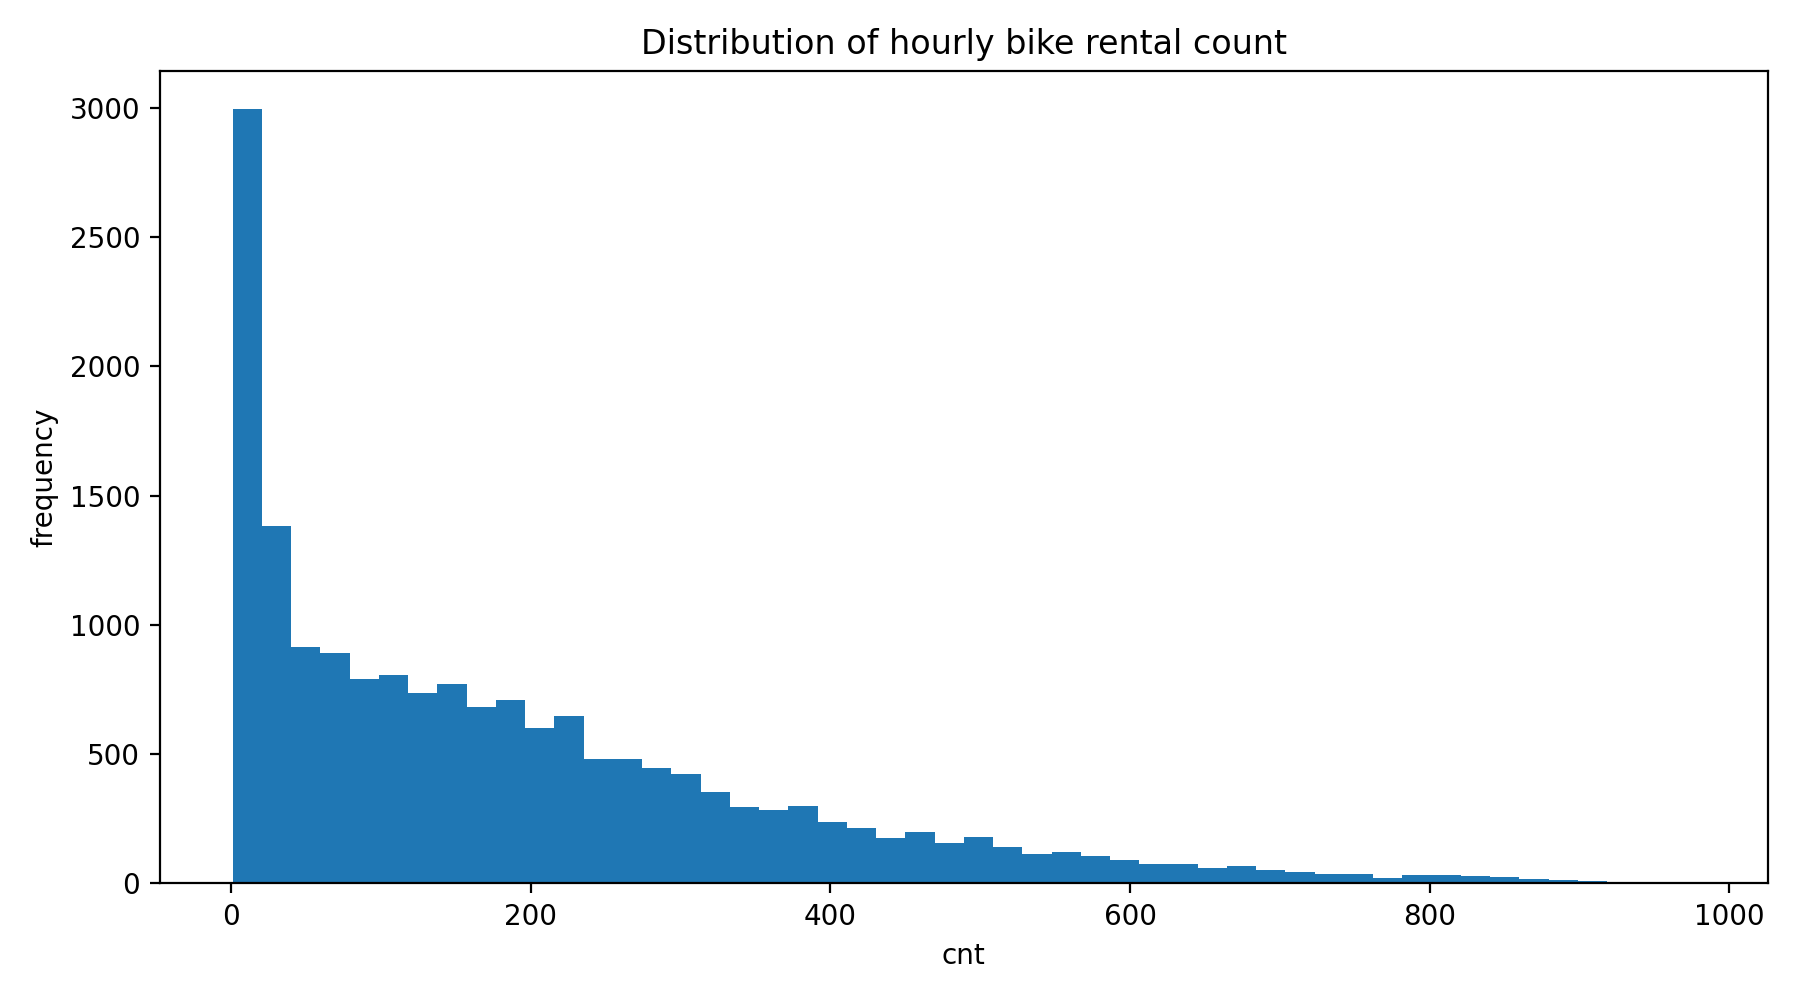
\includegraphics[width=0.88\linewidth]{figures/target_cnt_distribution.png}
    \caption{每小时共享单车租借总数分布}
    \label{fig:cntdist}
\end{figure}

图 \ref{fig:cntdist} 显示，大量小时的租借数量集中在较低区间，而高租借量样本相对较少。这种长尾分布说明不同时间段的需求差异显著，也解释了为什么对目标变量进行对数变换可能有助于改善部分模型表现。

\begin{figure}[H]
    \centering
    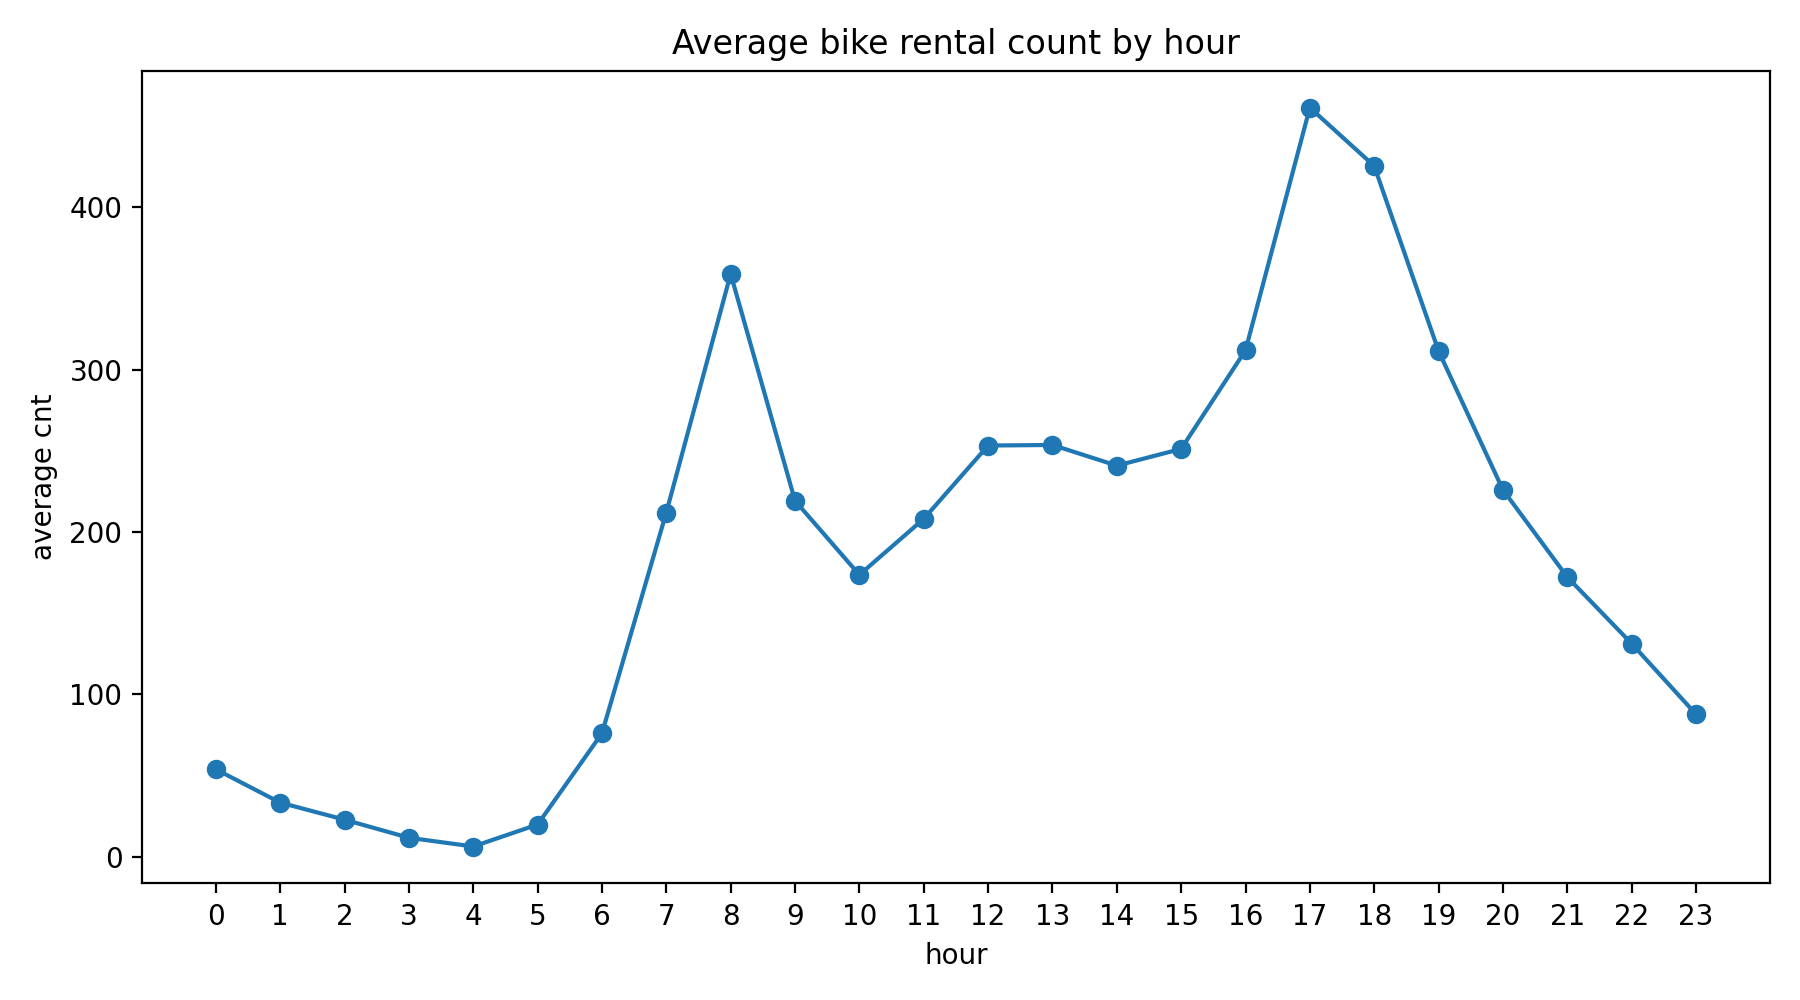
\includegraphics[width=0.86\linewidth]{figures/average_cnt_by_hour.png}
    \caption{不同小时的平均租借数量}
    \label{fig:houravg}
\end{figure}

从图 \ref{fig:houravg} 可以看到，租借数量具有明显小时周期规律。凌晨时段需求较低，白天逐步上升，并在通勤相关时段出现较高租借量。这说明小时特征是本任务中非常重要的预测变量。

\subsection{算法实现}

实验流程如下：
\begin{enumerate}
    \item 使用 \texttt{pandas} 读取 \texttt{hour.csv}，将 \texttt{dteday} 转换为日期格式，并与 \texttt{hr} 合成 \texttt{datetime}。
    \item 按时间顺序排序数据，使用前 80\% 样本作为训练集，后 20\% 样本作为测试集，避免时间序列场景中的未来信息泄漏。
    \item 进行数据预览，保存前 10 行数据、数据类型、描述性统计、缺失值统计、目标变量分布图和每小时平均租借量图。
    \item 计算数值字段相关系数，分析各特征与 \texttt{cnt} 的关系，并识别 \texttt{casual}、\texttt{registered} 这类目标泄漏字段。
    \item 直接建模阶段删除 \texttt{cnt}、\texttt{datetime}、\texttt{dteday}、\texttt{instant}、\texttt{casual} 和 \texttt{registered}，使用原始可用特征训练 Ridge 和 RandomForest 模型。
    \item 特征工程阶段构造日期、周期、分箱、业务逻辑和交互特征，包括 \texttt{hr\_sin}、\texttt{hr\_cos}、\texttt{is\_night}、\texttt{is\_peak\_hour}、\texttt{temp\_hum\_interaction} 等。
    \item 对类别特征进行 One-Hot 编码，对连续数值特征进行 IQR 异常值裁剪和 StandardScaler 标准化，对二值特征直接保留。
    \item 重新训练特征工程后的 Ridge 和 RandomForest 模型，输出模型评价指标、最佳模型预测曲线和随机森林特征重要性。
\end{enumerate}

评价指标中，RMSE 定义为
\begin{equation}
    RMSE=\sqrt{\frac{1}{n}\sum_{i=1}^{n}(\hat{y}^{(i)}-y^{(i)})^2},
\end{equation}
MAE 定义为
\begin{equation}
    MAE=\frac{1}{n}\sum_{i=1}^{n}\left|\hat{y}^{(i)}-y^{(i)}\right|,
\end{equation}
决定系数 $R^2$ 定义为
\begin{equation}
    R^2=1-\frac{\sum_{i=1}^{n}(y^{(i)}-\hat{y}^{(i)})^2}{\sum_{i=1}^{n}(y^{(i)}-\bar{y})^2}.
\end{equation}
完整 Python 程序见附录。

\section{实验结果与可扩展内容}

\subsection{实验结果}

相关性分析结果表明，若包含统计字段，\texttt{registered} 与 \texttt{cnt} 的相关系数为 0.9722，\texttt{casual} 与 \texttt{cnt} 的相关系数为 0.6946。但二者是目标变量的组成部分，不能用于实际预测。去除泄漏字段后，与目标关系较明显的字段包括 \texttt{temp}、\texttt{atemp}、\texttt{hr} 和 \texttt{hum}，其中温度和小时与租借量正相关，湿度与租借量负相关。

\begin{figure}[H]
    \centering
    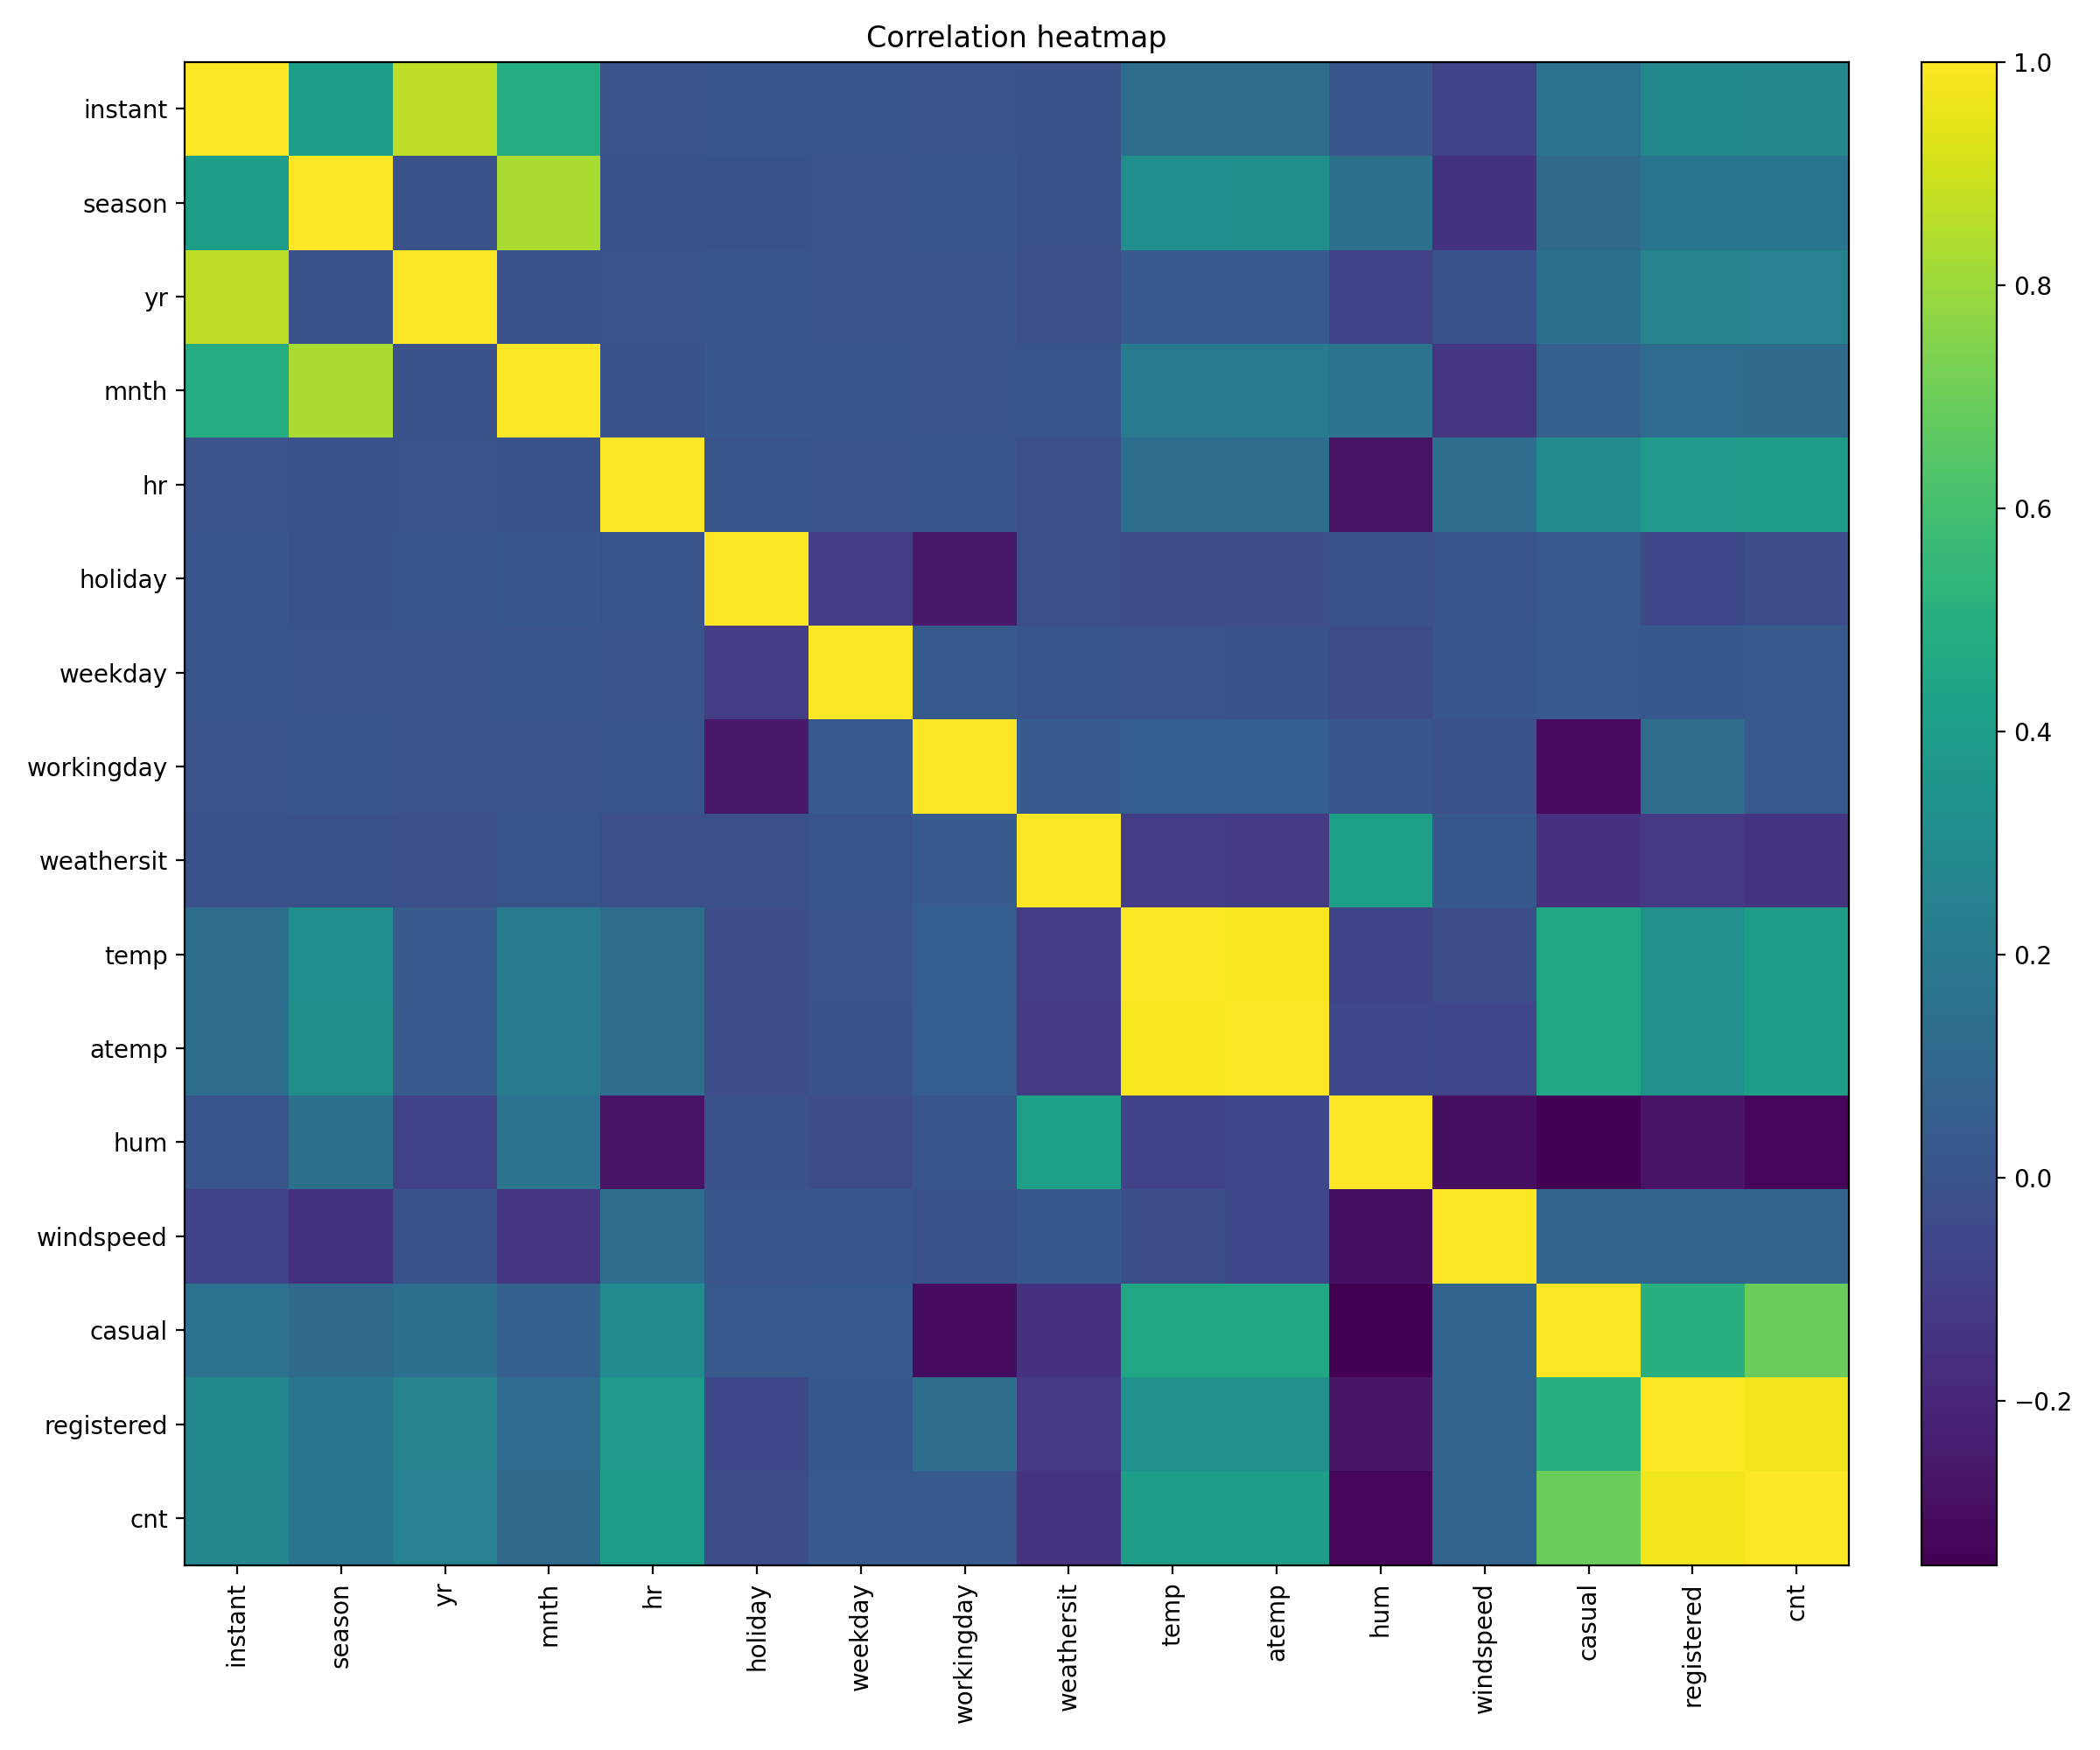
\includegraphics[width=0.82\linewidth]{figures/correlation_heatmap.png}
    \caption{数值字段相关性热力图}
    \label{fig:corr}
\end{figure}

直接建模阶段使用原始可用字段进行训练，结果见表 \ref{tab:direct-result}。在未进行复杂特征工程的情况下，随机森林已经取得较好效果，RMSE 为 69.90，MAE 为 45.02，测试集 $R^2$ 为 0.8995；而 Ridge 线性模型即使使用目标对数变换，$R^2$ 仅为 0.1520，说明原始编码下的线性模型难以充分刻画租借数量的非线性规律。

\begin{table}[H]
\centering
\caption{直接建模阶段模型结果}
\label{tab:direct-result}
\begin{tabular}{lcccc}
\toprule
模型 & RMSE & MAE & $R^2$ & NRMSE\\
\midrule
\texttt{Direct\_RandomForest} & 69.90 & 45.02 & 0.8995 & 0.0716\\
\texttt{Direct\_Ridge\_logTarget} & 203.04 & 139.83 & 0.1520 & 0.2080\\
\bottomrule
\end{tabular}
\end{table}

\begin{figure}[H]
    \centering
    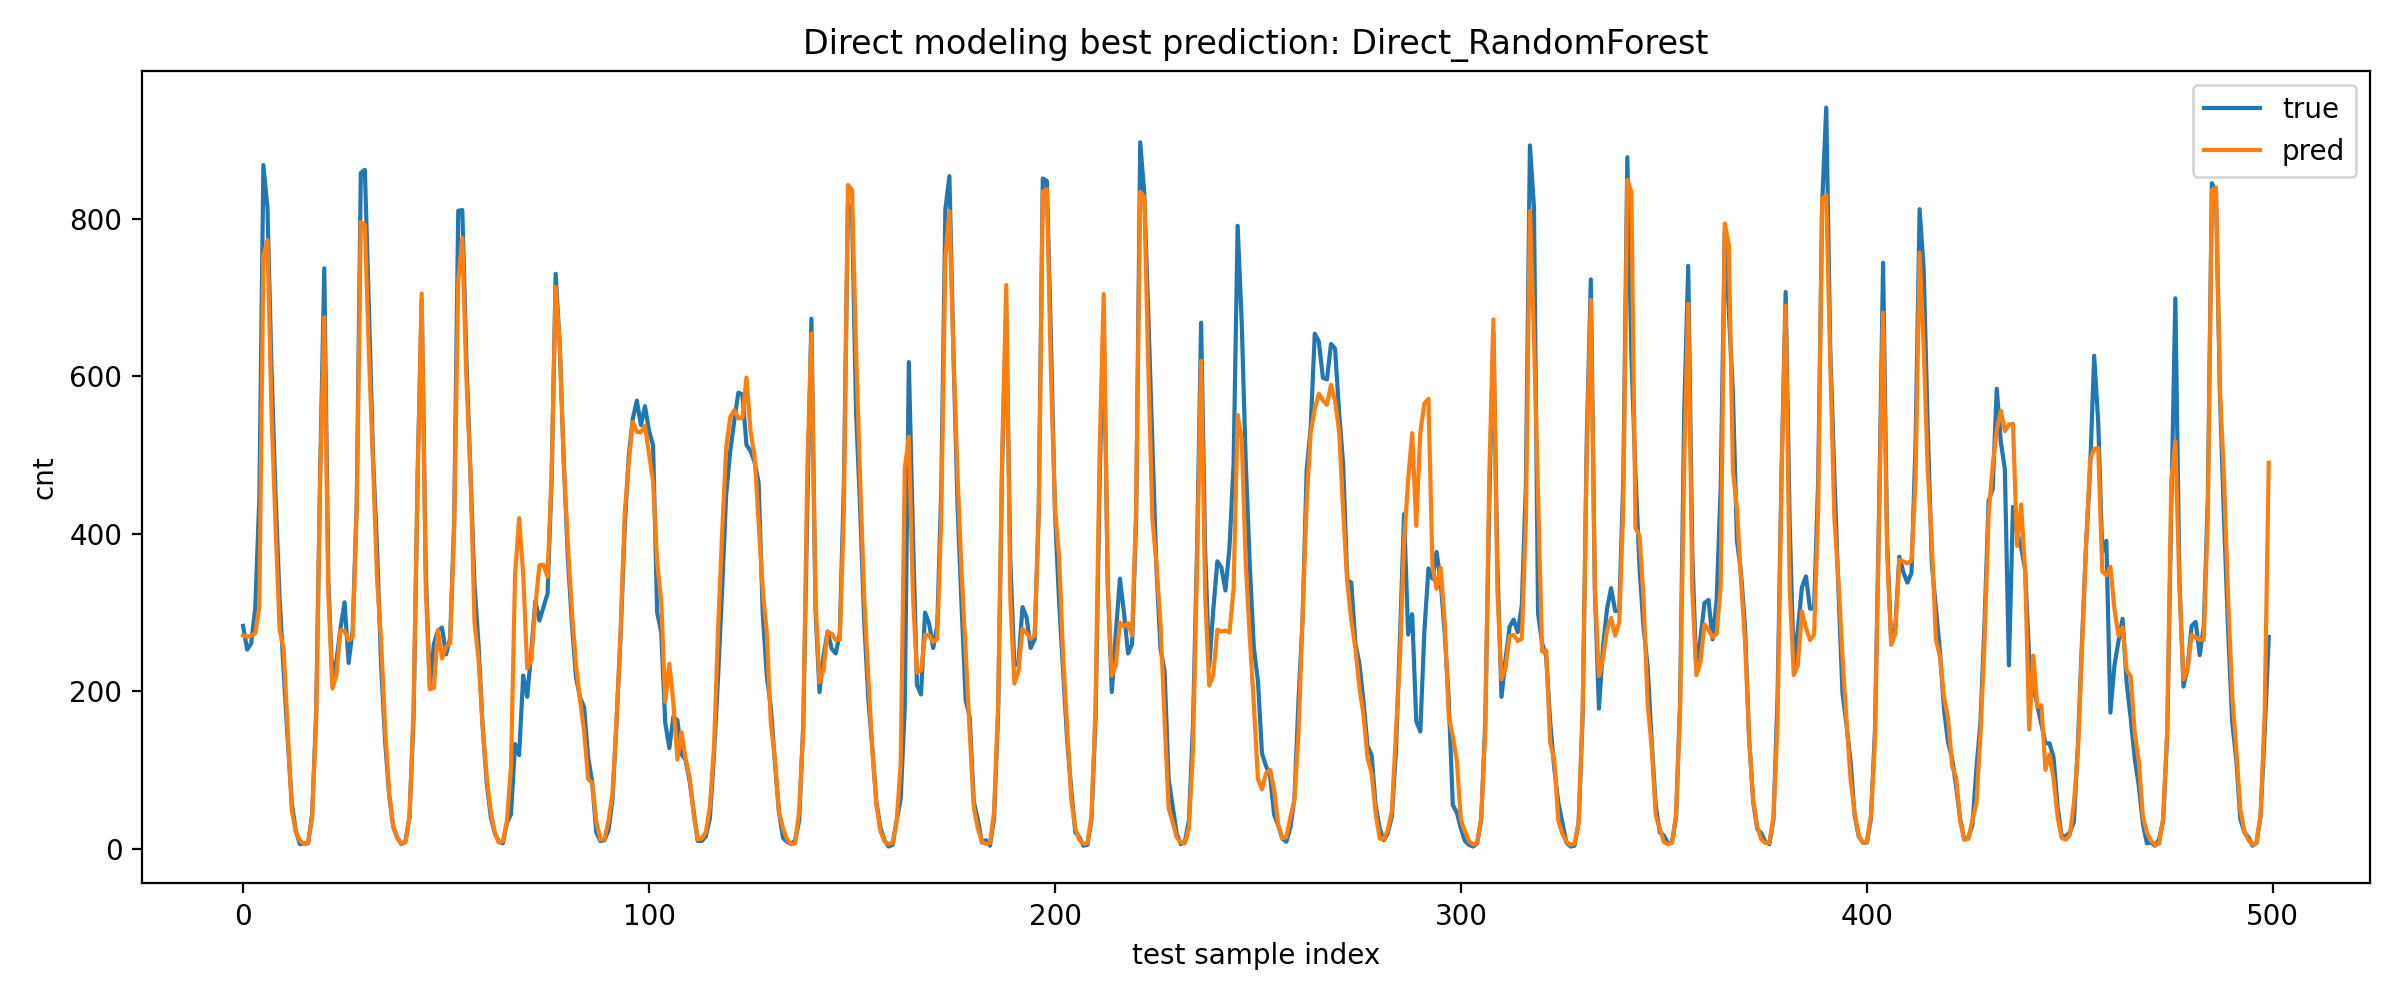
\includegraphics[width=0.9\linewidth]{figures/direct_best_prediction_curve.png}
    \caption{直接建模最佳模型预测曲线}
    \label{fig:directpred}
\end{figure}

图 \ref{fig:directpred} 展示了直接建模阶段最佳模型在测试集前 500 个样本上的预测效果。整体趋势能够跟随真实租借数量变化，但在部分峰值处仍存在低估或滞后现象，这与共享单车需求的突发波动有关。

特征工程阶段构造了日期、周期、分箱、通勤、天气和交互特征，并对连续变量进行异常值处理。IQR 检测结果显示，原始连续气象变量中 \texttt{windspeed} 在训练集有 91 个异常值、测试集有 16 个异常值；构造特征中 \texttt{feel\_temp\_diff}、\texttt{temp\_wind\_interaction} 和 \texttt{hum\_wind\_interaction} 的异常值较多，因此使用训练集计算上下界并同时裁剪训练集和测试集，避免测试集信息泄漏。

\begin{table}[H]
\centering
\caption{主要异常值裁剪结果}
\label{tab:outlier}
\begin{tabular}{lrrrr}
\toprule
特征 & 下界 & 上界 & 训练异常数 & 测试异常数\\
\midrule
\texttt{windspeed} & -0.1642 & 0.5523 & 91 & 16\\
\texttt{feel\_temp\_diff} & -0.0961 & 0.0567 & 392 & 61\\
\texttt{temp\_wind\_interaction} & -0.0921 & 0.2744 & 322 & 42\\
\texttt{hum\_wind\_interaction} & -0.0596 & 0.2809 & 426 & 77\\
\bottomrule
\end{tabular}
\end{table}

经过特征工程、编码、离散化、异常值处理和标准化之后，重新建模结果见表 \ref{tab:engineered-result}。随机森林在特征工程后测试集 $R^2$ 为 0.8774，仍保持较高水平；Ridge 模型提升非常明显，$R^2$ 从直接建模阶段的 0.1520 提升至 0.8055，说明特征编码、周期特征和标准化对线性模型帮助很大。

\begin{table}[H]
\centering
\caption{特征工程后重新建模结果}
\label{tab:engineered-result}
\begin{tabular}{lcccc}
\toprule
模型 & RMSE & MAE & $R^2$ & NRMSE\\
\midrule
\texttt{FE\_RandomForest\_logTarget} & 77.20 & 50.69 & 0.8774 & 0.0791\\
\texttt{FE\_Ridge\_logTarget} & 97.23 & 61.15 & 0.8055 & 0.0996\\
\bottomrule
\end{tabular}
\end{table}

\begin{figure}[H]
    \centering
    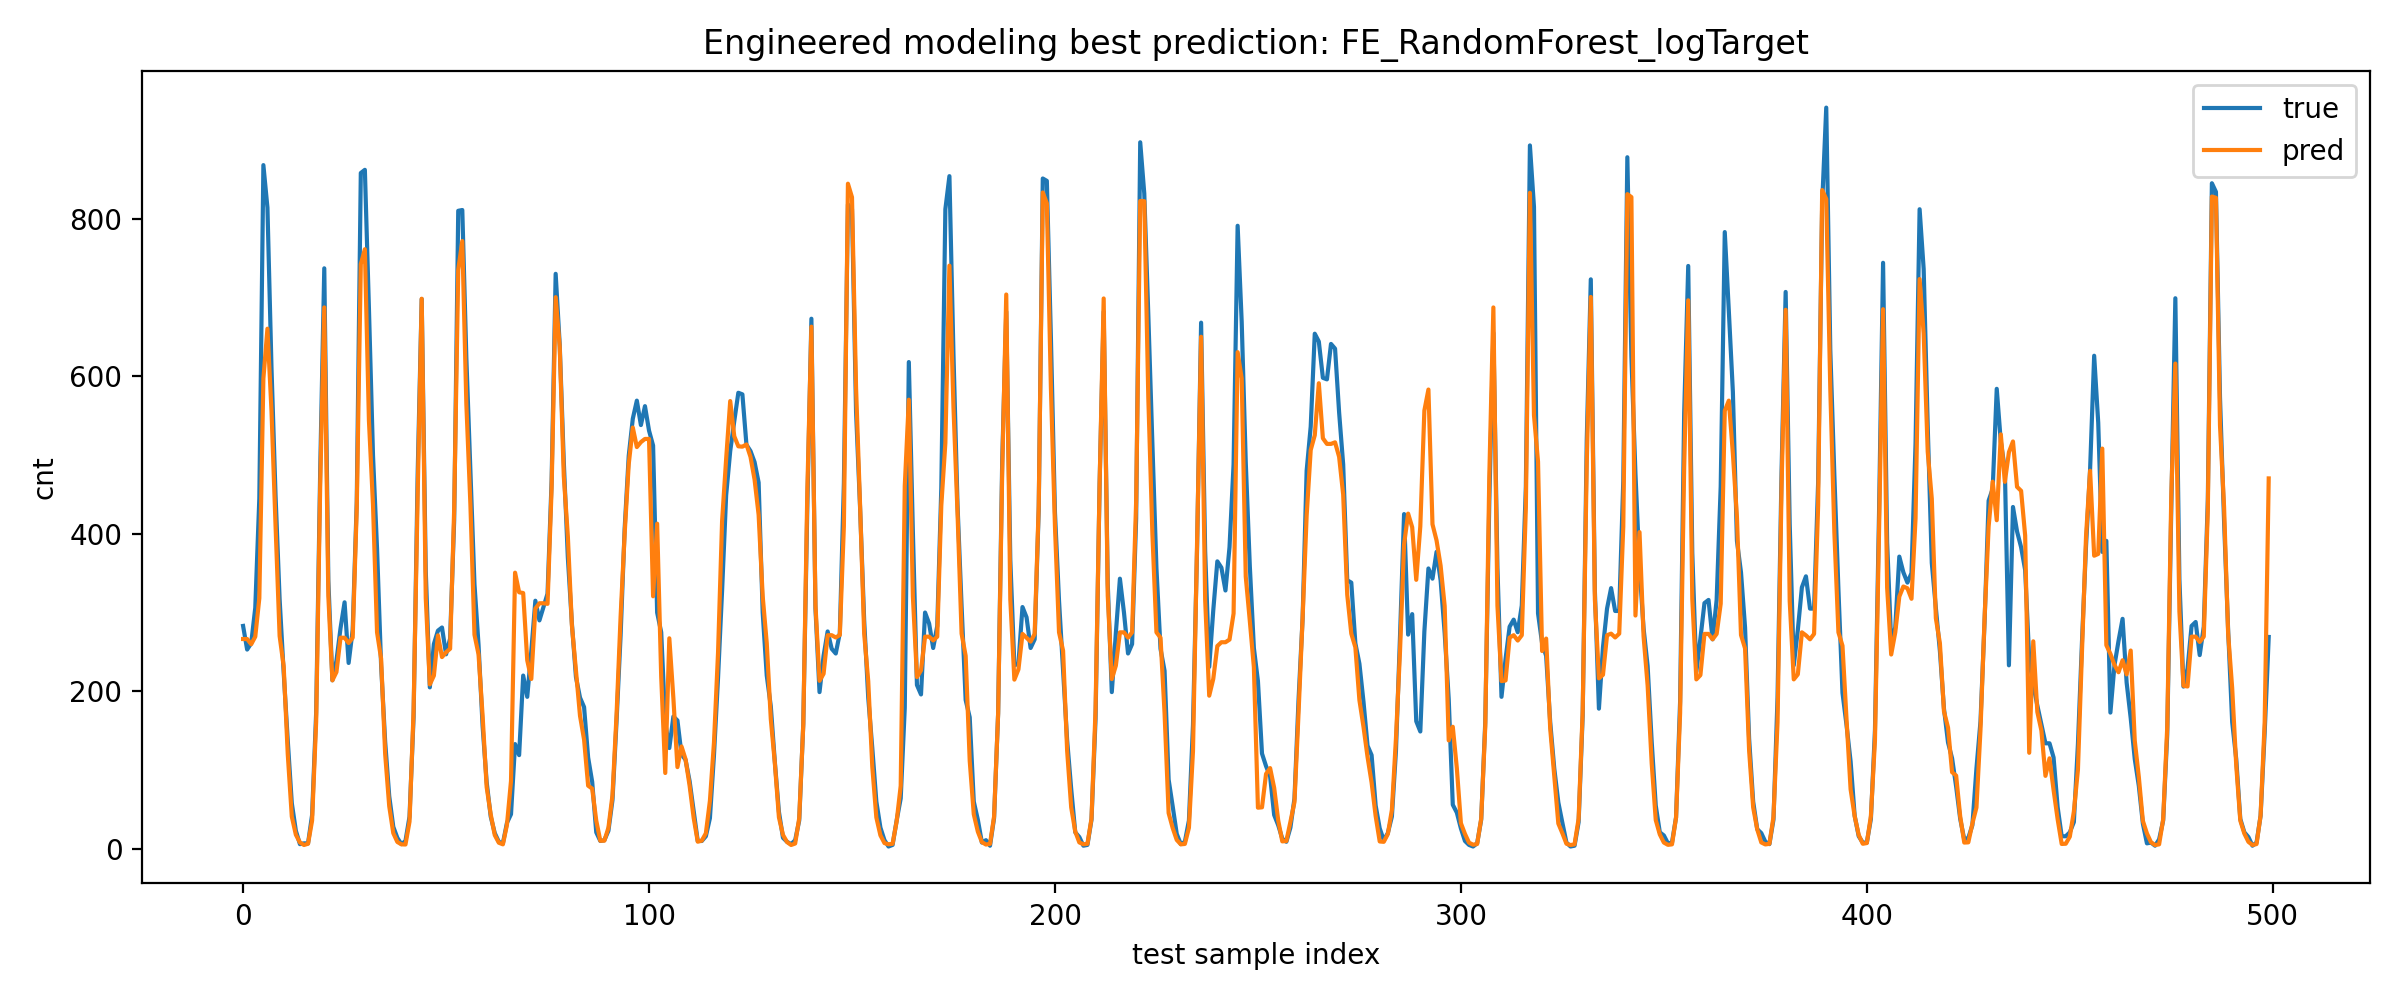
\includegraphics[width=0.9\linewidth]{figures/engineered_best_prediction_curve.png}
    \caption{特征工程后最佳模型预测曲线}
    \label{fig:fepred}
\end{figure}

将所有模型进行汇总，直接随机森林取得本次实验中最低 RMSE 和最高 $R^2$，是整体最优模型；特征工程后的随机森林略低于直接随机森林，可能与模型参数设置不同、目标对数变换以及特征处理方式有关。但从线性模型角度看，特征工程后的 Ridge 表现大幅改善，说明预处理流程本身是有效的。

\begin{table}[H]
\centering
\caption{全部模型对比结果}
\label{tab:all-result}
\begin{tabular}{lcccl}
\toprule
模型 & RMSE & MAE & $R^2$ & 阶段\\
\midrule
\texttt{Direct\_RandomForest} & 69.90 & 45.02 & 0.8995 & 直接建模\\
\texttt{FE\_RandomForest\_logTarget} & 77.20 & 50.69 & 0.8774 & 特征工程后\\
\texttt{FE\_Ridge\_logTarget} & 97.23 & 61.15 & 0.8055 & 特征工程后\\
\texttt{Direct\_Ridge\_logTarget} & 203.04 & 139.83 & 0.1520 & 直接建模\\
\bottomrule
\end{tabular}
\end{table}

\subsection{参数调优及可扩展内容}

随机森林特征重要性结果见图 \ref{fig:importance}。其中 \texttt{is\_night} 重要性最高，为 0.4919；\texttt{hr\_sin} 重要性为 0.1916；随后是 \texttt{temp}、\texttt{is\_peak\_hour}、\texttt{atemp} 和 \texttt{hr\_cos}。这说明小时周期、夜间判断、通勤高峰和温度是预测每小时租借数量的关键因素。

\begin{figure}[H]
    \centering
    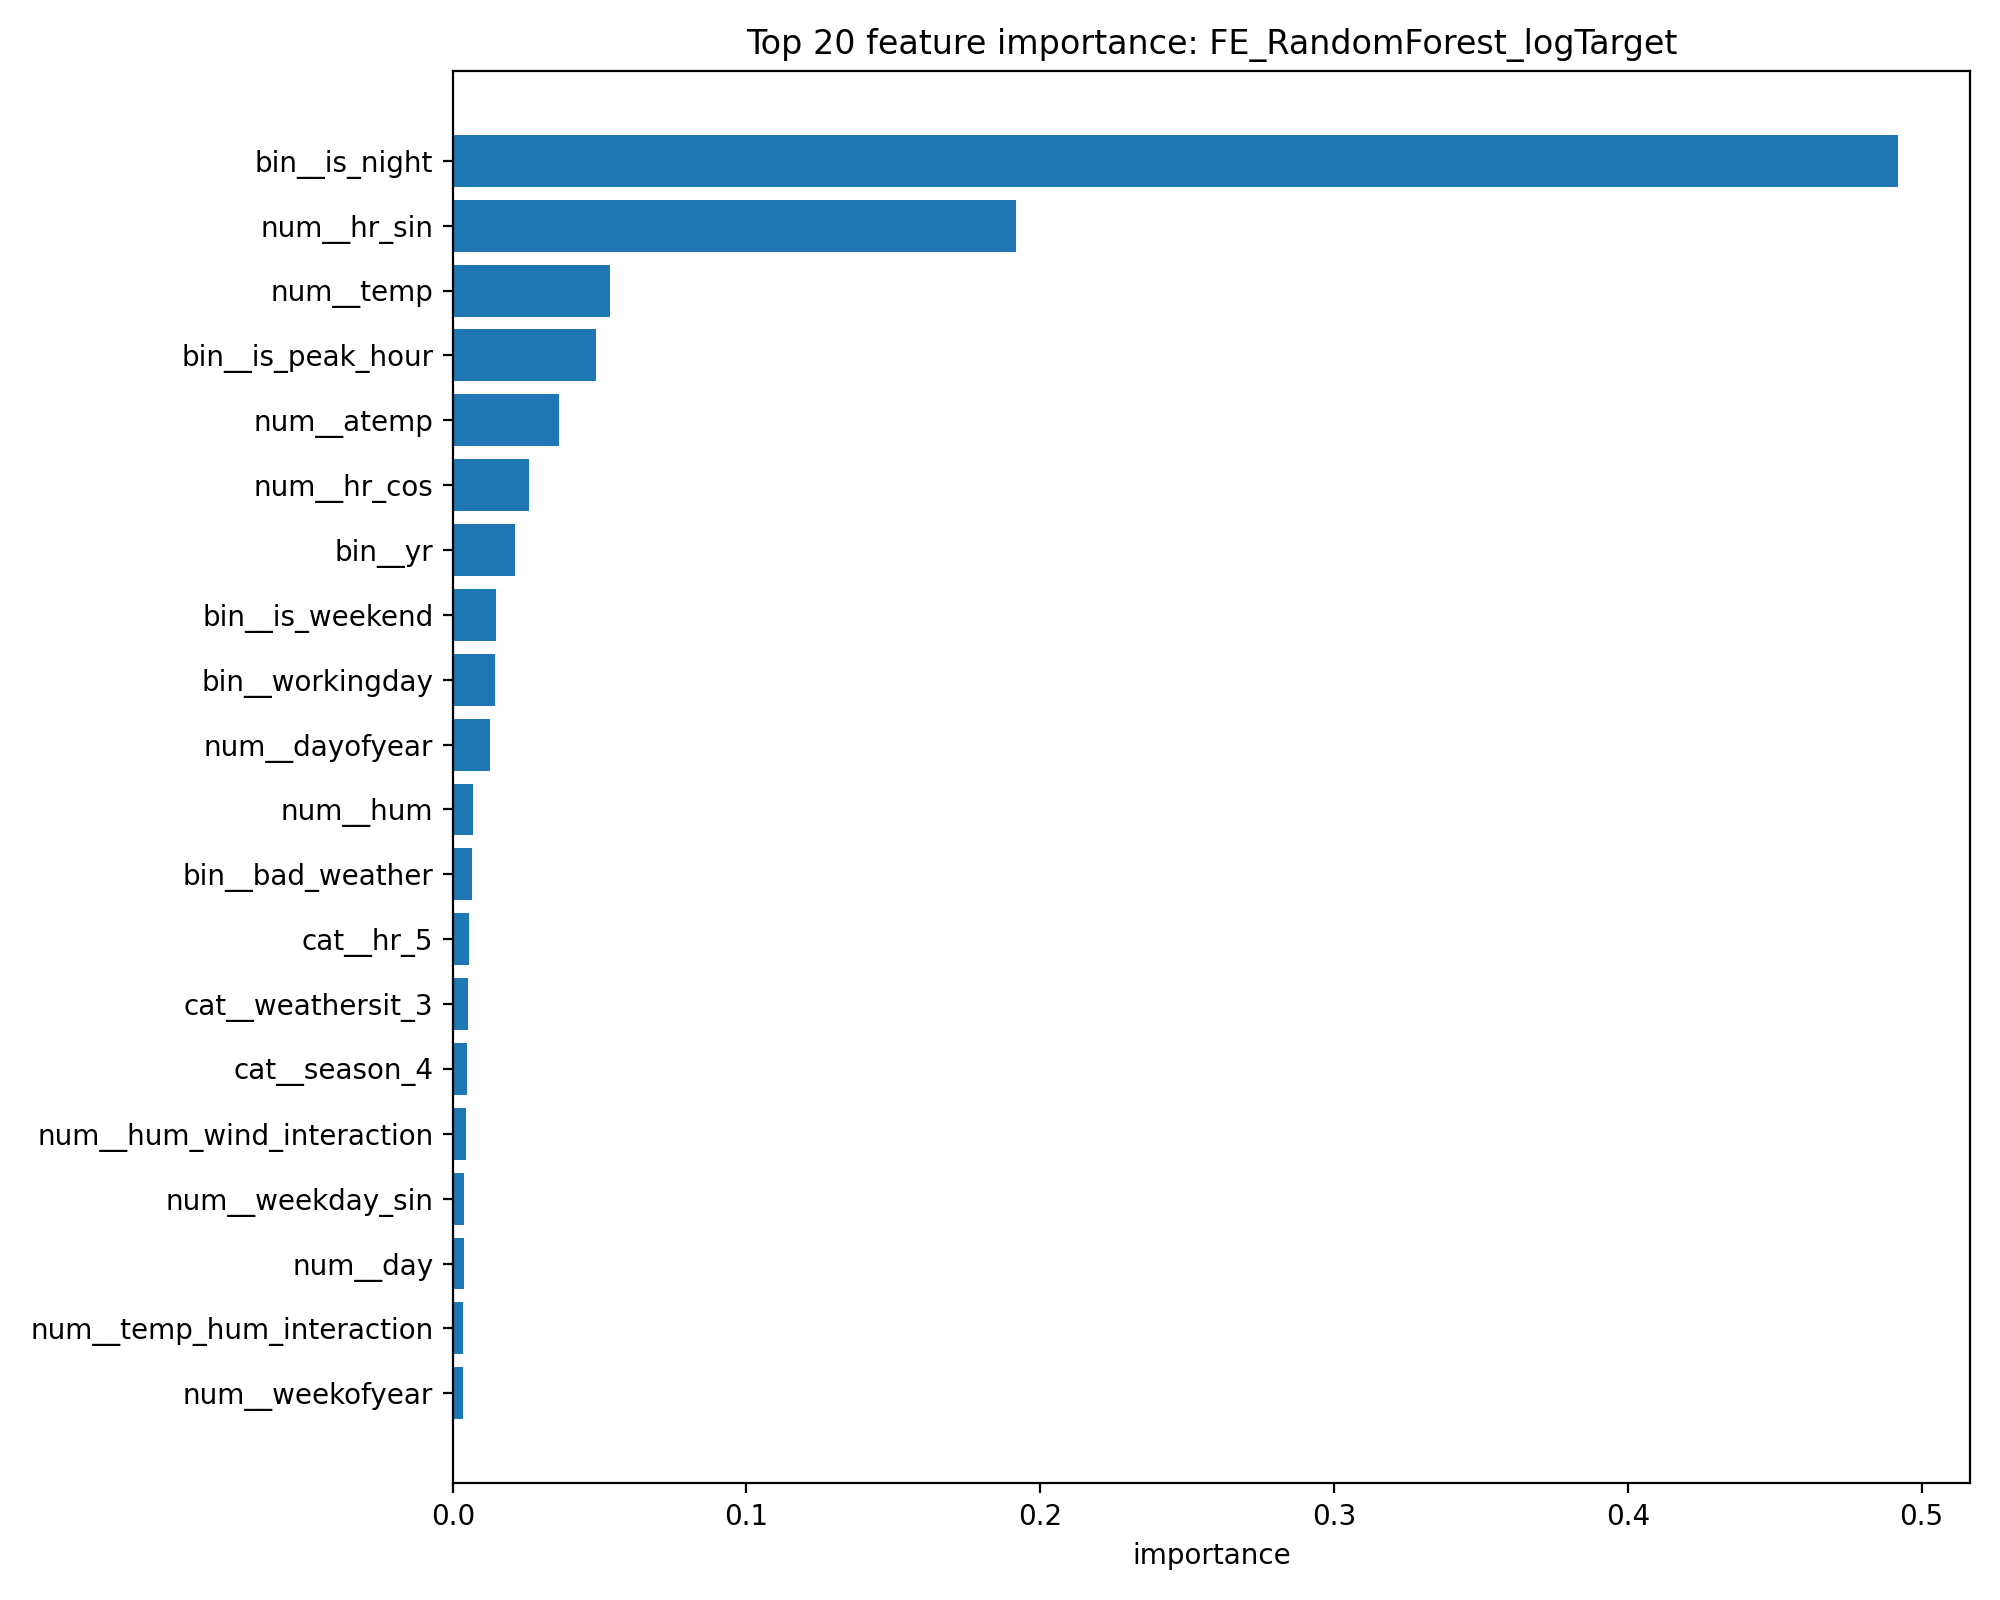
\includegraphics[width=0.9\linewidth]{figures/feature_importance_top20.png}
    \caption{特征工程后随机森林前 20 个重要特征}
    \label{fig:importance}
\end{figure}

根据当前结果，后续可以从以下方向继续扩展。第一，可以对随机森林的 \texttt{n\_estimators}、\texttt{max\_depth}、\texttt{min\_samples\_leaf} 等参数进行网格搜索或随机搜索，寻找更稳定的泛化效果。第二，可以尝试 Gradient Boosting、XGBoost 或 LightGBM 等提升树模型，这类模型通常对表格型数据表现较好。第三，可以增加滚动时间窗口特征，例如过去 24 小时平均租借量、上一天同小时租借量等，以更充分利用时间序列信息。第四，可以分别预测 \texttt{casual} 与 \texttt{registered} 后再相加，从而刻画休闲用户和通勤用户不同的出行规律。

\section{讨论与结论}

\subsection{结果讨论}

通过实验可以得到以下结论。第一，共享单车小时租借数量具有明显时间周期性。凌晨需求最低，白天和通勤时段需求更高，因此小时特征及其周期编码是本任务中的核心信息。特征重要性中 \texttt{is\_night}、\texttt{hr\_sin} 和 \texttt{hr\_cos} 排名靠前，也验证了这一点。

第二，目标泄漏字段必须严格排除。\texttt{casual} 和 \texttt{registered} 与 \texttt{cnt} 高度相关，但它们本身就是目标变量的组成部分。若将其作为输入，模型会得到虚假的高精度，无法用于真实预测场景。本实验在建模阶段删除这两个字段，使评价结果更符合实际使用要求。

第三，树模型比简单线性模型更适合本任务。直接随机森林在原始可用特征上取得 $R^2=0.8995$，说明它能够自动学习非线性划分和变量交互。相比之下，直接 Ridge 模型表现较差，说明仅用原始数值编码的线性关系不足以描述租借需求。

第四，预处理和特征工程对线性模型提升明显。经过 One-Hot 编码、周期特征、离散化、业务特征、异常值裁剪和标准化之后，Ridge 的 $R^2$ 提升到 0.8055。虽然该结果仍低于随机森林，但已经能较好解释租借数量变化，说明规范的数据预处理流程可以显著增强模型表达能力。

\subsection{结论总结}

本次实验完成了基于共享单车小时数据的租借数量预测任务。实验从数据预览和相关分析出发，先建立直接建模基线，再按照题目要求完成特征工程、特征编码、离散化、新特征构造、异常值处理、数值标准化和重新建模。最终结果显示，直接随机森林模型表现最好，RMSE 为 69.90，MAE 为 45.02，$R^2$ 为 0.8995；特征工程后的 Ridge 模型相较直接 Ridge 有大幅提升，证明预处理过程对模型效果具有重要影响。

综合来看，共享单车需求预测不仅需要选择合适模型，也依赖于对数据含义的理解。时间、天气、工作日、通勤高峰和夜间等因素都与租借数量密切相关。通过本案例，可以较系统地理解回归预测任务中从数据预处理到模型评价的完整流程。

\section{心得体会与思考}

\subsection{个人心得}

通过本次实验，我对数据预处理在机器学习中的作用有了更直观的认识。模型训练并不是简单地把所有字段输入算法，而是需要先判断字段是否可用、是否存在泄漏、是否需要编码和标准化。例如 \texttt{casual} 与 \texttt{registered} 虽然和目标高度相关，但在真实预测中不能提前知道，因此必须删除。

同时，我也体会到不同模型对特征处理的依赖程度不同。随机森林能够较好处理非线性和交互关系，因此直接建模就能取得较好结果；而 Ridge 等线性模型更依赖合理的编码、标准化和特征构造。这个对比让我更清楚地理解了模型能力与特征工程之间的关系。

\subsection{启发与思考}

共享单车租借量受到时间、天气和用户出行习惯共同影响，是一个具有明显业务背景的预测问题。仅从相关系数或单个字段出发很难完全解释需求变化，必须结合工作日、通勤时间、夜间、天气好坏和温湿度交互等因素综合建模。

后续如果继续改进，可以把问题进一步扩展为时间序列预测任务，引入滞后特征和滚动统计特征；也可以尝试更强的集成学习模型，并通过交叉验证或按月份滚动验证评估模型稳定性。这样不仅可以提升预测精度，也能更接近实际共享单车运营中的调度场景。

\section{附录}

\subsection*{算法代码及其注释}
\addcontentsline{toc}{subsection}{算法代码及其注释}

\VerbatimInput[breaklines,breakanywhere,fontsize=\small,frame=single,rulecolor=\color{gray!45}]{report_code.py}

\subsection*{关键运行结果汇总}
\addcontentsline{toc}{subsection}{关键运行结果汇总}

报告2中记录的主要运行结果如下：

\begin{CodeBlock}
数据规模：
17379 行，18 列；所有字段缺失值数量均为 0。

直接建模：
Direct_RandomForest        RMSE=69.9025,  MAE=45.0211,  R2=0.8995, NRMSE=0.0716
Direct_Ridge_logTarget     RMSE=203.0361, MAE=139.8291, R2=0.1520, NRMSE=0.2080

特征工程后建模：
FE_RandomForest_logTarget  RMSE=77.2029, MAE=50.6933, R2=0.8774, NRMSE=0.0791
FE_Ridge_logTarget         RMSE=97.2286, MAE=61.1494, R2=0.8055, NRMSE=0.0996

重要特征：
is_night=0.4919, hr_sin=0.1916, temp=0.0534,
is_peak_hour=0.0487, atemp=0.0362, hr_cos=0.0261。
\end{CodeBlock}

\end{document}
